\documentclass[tikz,border=10pt]{standalone}
\usepackage{amsmath}
\usetikzlibrary{arrows.meta, positioning, calc}

\begin{document}
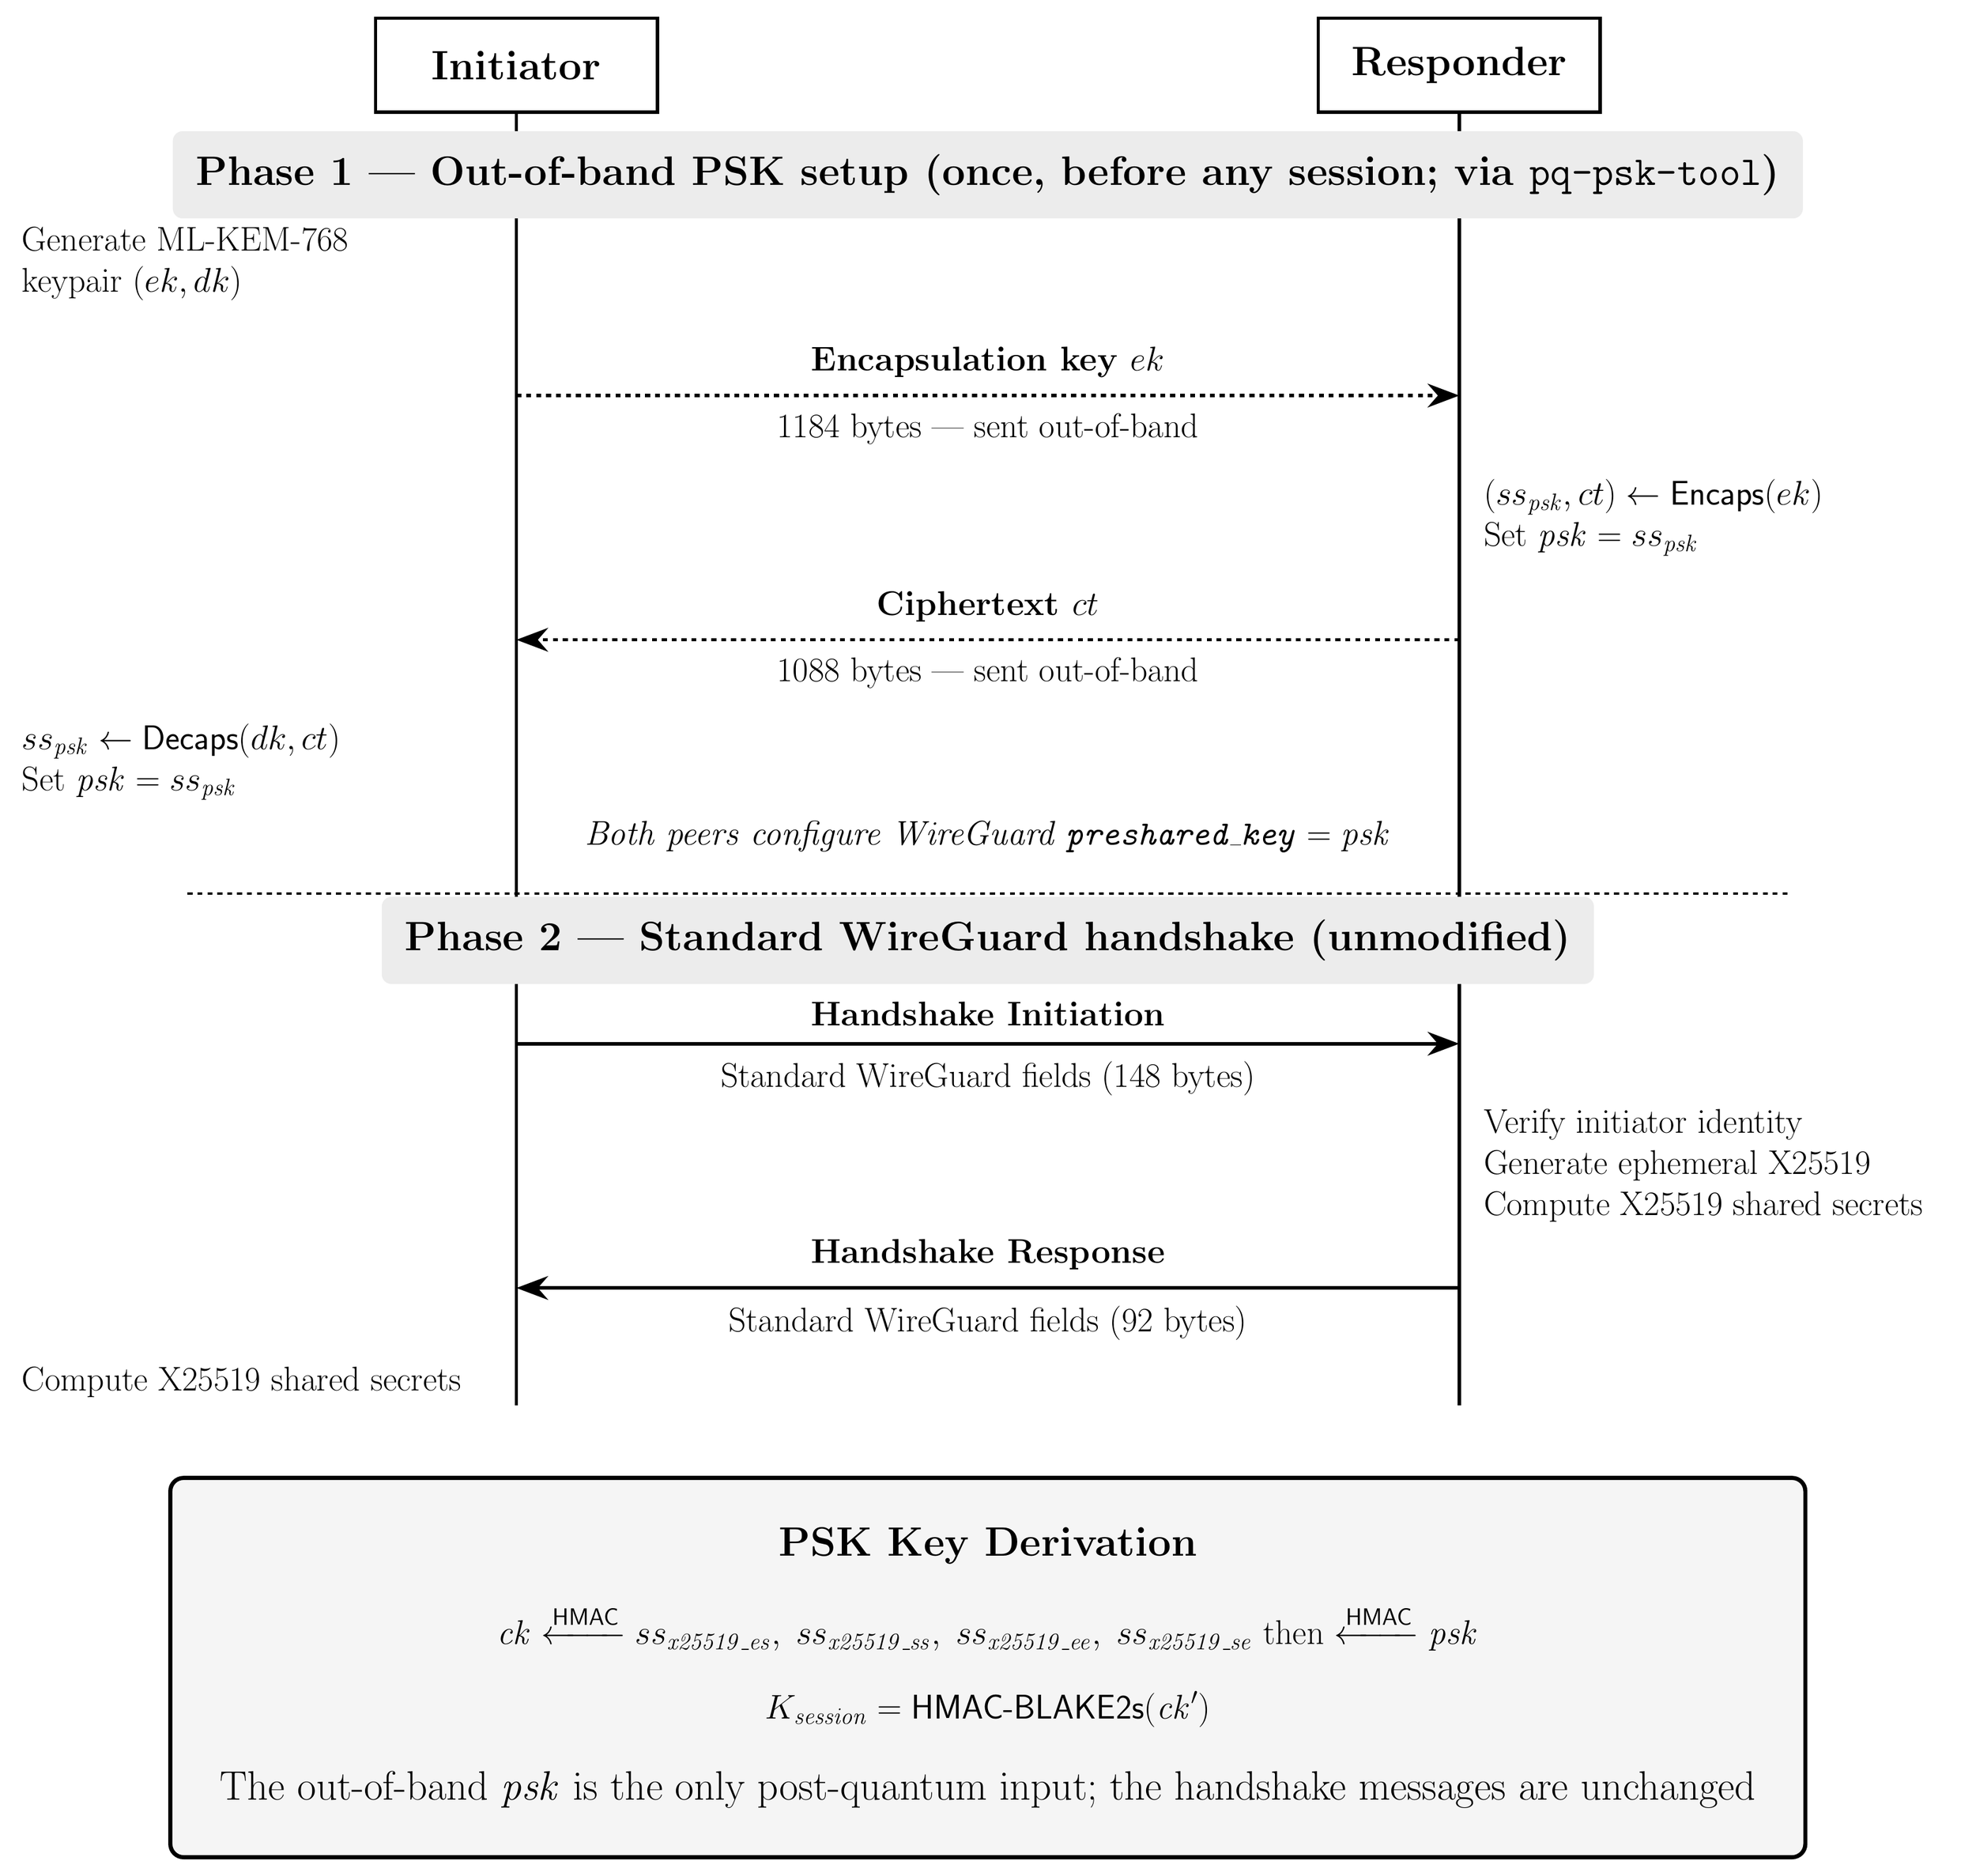
\begin{tikzpicture}[
    box/.style={rectangle, draw=black, line width=2pt, minimum width=6cm, minimum height=2cm, align=center, font=\bfseries\Huge},
    arrow/.style={-{Stealth[scale=1.6]}, line width=2pt},
    ooba/.style={-{Stealth[scale=1.6]}, line width=2pt, dashed},
    msg_label/.style={font=\huge\bfseries, fill=white, inner sep=5pt},
    msg_detail/.style={font=\huge, fill=white, inner sep=5pt},
    action/.style={font=\huge, text width=10cm, align=left},
    note/.style={font=\huge\itshape, fill=white, align=center, inner sep=8pt},
    phase/.style={font=\Huge\bfseries, fill=gray!15, rounded corners=6pt, inner sep=14pt},
    timeline/.style={line width=2pt}
]
    % Spacing constants
    \def\colsep{14cm}

    % Nodes
    \node[box] (init) {Initiator};
    \node[box, right=\colsep of init] (resp) {Responder};

    % Timelines
    \draw[timeline] (init.south) -- +(0,-27.5cm);
    \draw[timeline] (resp.south) -- +(0,-27.5cm);

    % ===================== PHASE 1: OUT-OF-BAND PSK SETUP =====================
    \node[phase] (p1) at ($(init.south)!0.5!(resp.south)-(0,1.3cm)$)
        {Phase 1 --- Out-of-band PSK setup (once, before any session; via \texttt{pq-psk-tool})};

    % P1a: Initiator generates ML-KEM keypair
    \coordinate (p1a) at ($(init.south)-(0,3.2cm)$);
    \node[action, anchor=east] at ($(p1a)+(-0.4cm,0)$) {Generate ML-KEM-768\\keypair $(ek, dk)$};

    % P1 msg 1: send ek (out-of-band)
    \coordinate (e1_start) at ($(init.south)-(0,6cm)$);
    \coordinate (e1_end) at ($(resp.south)-(0,6cm)$);
    \draw[ooba] (e1_start) -- (e1_end);
    \node[msg_label, above=0.2cm] at ($(e1_start)!0.5!(e1_end)$) {Encapsulation key $ek$};
    \node[msg_detail, below=0.2cm] at ($(e1_start)!0.5!(e1_end)$) {1184 bytes --- sent out-of-band};

    % P1b: Responder encapsulates
    \coordinate (p1b) at ($(resp.south)-(0,8.6cm)$);
    \node[action, anchor=west] at ($(p1b)+(0.4cm,0)$) {$(ss_{\mathit{psk}}, ct) \gets \textsf{Encaps}(ek)$\\Set $\mathit{psk} = ss_{\mathit{psk}}$};

    % P1 msg 2: send ct back (out-of-band)
    \coordinate (e2_start) at ($(resp.south)-(0,11.2cm)$);
    \coordinate (e2_end) at ($(init.south)-(0,11.2cm)$);
    \draw[ooba] (e2_start) -- (e2_end);
    \node[msg_label, above=0.2cm] at ($(e2_start)!0.5!(e2_end)$) {Ciphertext $ct$};
    \node[msg_detail, below=0.2cm] at ($(e2_start)!0.5!(e2_end)$) {1088 bytes --- sent out-of-band};

    % P1c: Initiator decapsulates
    \coordinate (p1c) at ($(init.south)-(0,13.8cm)$);
    \node[action, anchor=east] at ($(p1c)+(-0.4cm,0)$) {$ss_{\mathit{psk}} \gets \textsf{Decaps}(dk, ct)$\\Set $\mathit{psk} = ss_{\mathit{psk}}$};

    % Both configure the PSK slot
    \node[note] at ($(init.south)!0.5!(resp.south)-(0,15.4cm)$)
        {Both peers configure WireGuard \texttt{preshared\_key} $= \mathit{psk}$};

    % ===================== PHASE 2: WIREGUARD HANDSHAKE =====================
    \draw[dashed, line width=1.5pt] ($(init.south)-(7cm,16.6cm)$) -- ($(resp.south)+(7cm,0)-(0,16.6cm)$);
    \node[phase] at ($(init.south)!0.5!(resp.south)-(0,17.6cm)$)
        {Phase 2 --- Standard WireGuard handshake (unmodified)};

    % Msg 1: Handshake Initiation
    \coordinate (m1_start) at ($(init.south)-(0,19.8cm)$);
    \coordinate (m1_end) at ($(resp.south)-(0,19.8cm)$);
    \draw[arrow] (m1_start) -- (m1_end);
    \node[msg_label, above=0.2cm] at ($(m1_start)!0.5!(m1_end)$) {Handshake Initiation};
    \node[msg_detail, below=0.2cm] at ($(m1_start)!0.5!(m1_end)$) {Standard WireGuard fields (148 bytes)};

    % Responder processes
    \coordinate (r2) at ($(resp.south)-(0,22.4cm)$);
    \node[action, anchor=west] at ($(r2)+(0.4cm,0)$) {Verify initiator identity\\Generate ephemeral X25519\\Compute X25519 shared secrets};

    % Msg 2: Handshake Response
    \coordinate (m2_start) at ($(resp.south)-(0,25cm)$);
    \coordinate (m2_end) at ($(init.south)-(0,25cm)$);
    \draw[arrow] (m2_start) -- (m2_end);
    \node[msg_label, above=0.2cm] at ($(m2_start)!0.5!(m2_end)$) {Handshake Response};
    \node[msg_detail, below=0.2cm] at ($(m2_start)!0.5!(m2_end)$) {Standard WireGuard fields (92 bytes)};

    % Initiator computes X25519 shared secrets
    \coordinate (r3) at ($(init.south)-(0,27cm)$);
    \node[action, anchor=east] at ($(r3)+(-0.4cm,0)$) {Compute X25519 shared secrets};

    % PSK Key Derivation box
    \node[draw, line width=2.5pt, fill=gray!8, rounded corners=8pt, below=29cm of $(init.south)!0.5!(resp.south)$, anchor=north, align=center, inner sep=30pt, font=\huge] (kdf) {
        \textbf{\Huge PSK Key Derivation}\\[24pt]
        $\mathit{ck} \xleftarrow{\textsf{HMAC}} ss_{\mathit{x25519\_es}},\; ss_{\mathit{x25519\_ss}},\; ss_{\mathit{x25519\_ee}},\; ss_{\mathit{x25519\_se}}$ then $\xleftarrow{\textsf{HMAC}} \mathit{psk}$\\[20pt]
        $K_{\mathit{session}} = \textsf{HMAC-BLAKE2s}(\mathit{ck}')$\\[24pt]
        {\Huge The out-of-band $\mathit{psk}$ is the only post-quantum input; the handshake messages are unchanged}
    };

\end{tikzpicture}
\end{document}
